% !TeX root = ../main.tex

\chapter{DPU 测试日志}

\section{2023.11.15~第一次上电}

器件采购商将 LTM4644-1 发成 LTM4644 导致 DC-DC 输出电压不对,需修改值如下:
\begin{itemize}
  \item R675: 90.9k\qquad for 1.0V
  \item R678: 30.1k\qquad for 1.8V
  \item R684: 13.3k\qquad for 3.3V
  \item R691: 10k, R690: 68k\qquad for 2.5V
  \item R699: 60.4k\qquad for 1.2V
  \item R703: 12k, R702: 20k\qquad for 1.35V
  \item R707: 5.66k, R706: 60.4k\qquad for 3.8V
  \item R711: 3.9k, R710: 68k\qquad for 5.5V
  \item R674, R677, R683, R698 去掉, (LTM4644 已内置 60.4k)
\end{itemize}

绿色LED封装画反: D1, D26, D27, D28, D29, D30, D31, D32, D33, D41, D47, D48 \par
红色LED封装画反: D40, D42 \par
FT232HL做为Xilinx的JTAG时,需要往EEPROM里烧写数据。网址: \href{https://github.com/TerayTech/TT_Digilent_JTAG_HS2}{https://github.com/TerayTech/TT\_Digilent\_JTAG\_HS2}。 烧写频率默认为15000000, 可以正常烧写程序, 烧写ILA时报错, 需把频率调为7500000。\par

\section{2023.11.18~PLL调试}

LMK04610 的一路 VCC2.5VA 未提供,从TP8测试点飞线到 C395 左侧Pin1后,LMK04610 工作正常。
%修改的寄存器表如下:
%\inputminted{shell}{./figures/pll_rom.mem} \par

\section{2023.11.20~验证时钟配置}

\section{2023.11.21~Flash配置}
逻辑无法固化,检查原理图发现,U8 Flash 的 CS 信号错接到 U34 DS18S20 的 DQ 上,将U34 去掉后,将U8 的 7脚飞到 U34 的 4脚。\par
差分LEMO连接器无法插上,把D36、D37、D38、D39去掉即可。

%\section{2023.11.26~ADC 寄存器解读\textsl{}}
%\mintinline{shell}|0a3000|: Initialization after power-up. \par
%\mintinline{shell}|000000|: Register readout disabled \& Reset disabled. \par
%\mintinline{shell}|010060|: JESD interface enabled \& LVDS interface disabled \& 32-channel input. \par

\section{2024.01.09~FPGA GT Bank供电问题}
FPGA GT Bank供电不足,导致4片ADC无法同时工作。经检查发现,电源分配中,1.8VD 同时给 1.0VA 的 FPGA 内核和 1.2VA 的FPGA GT Bank 供电,用直流电源替换 1.8VD 的供电端,显示超过 LTM4644 的最大输出电流 4A。\par
尝试解决方案:\par
如图 \ref{fig:powersolution1},在U43器件周围,沿着绿色的画线,把表层的铜皮割断;然后再沿着蓝色的画线,把它们用飞线连上。最后用飞线将 C711 右侧的 1.2VD 供电端飞到 C683 右侧的管脚上。\par
\begin{figure}[htbp]
  \centering
  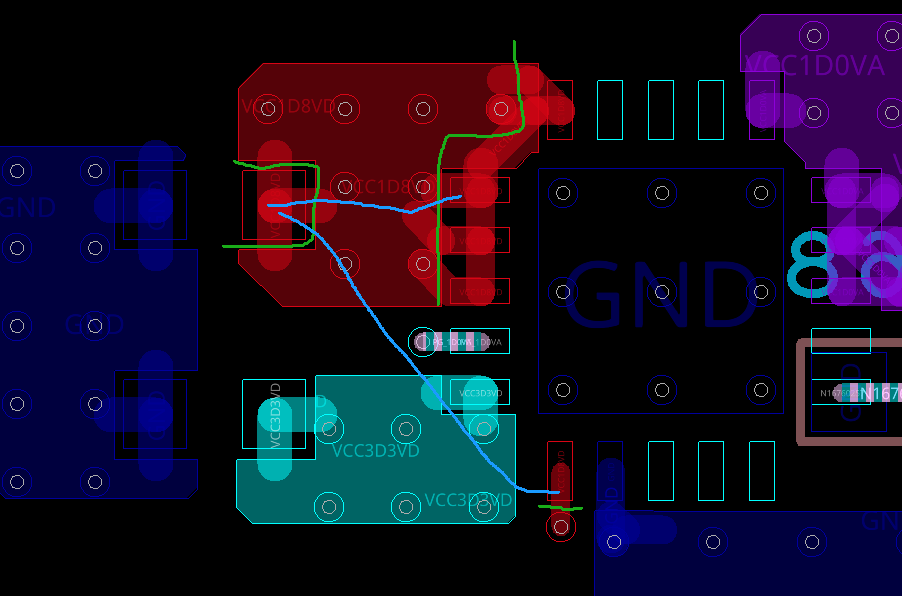
\includegraphics[width=0.65\textwidth]{powersolution1.png}
  \caption{电源解决方案1}
  \label{fig:powersolution1}
\end{figure}
来实现 FPGA 内核与 FPGA GT Bank 的分离供电。\par
为解决,仍然无法负载4个GT Bank,考虑后续改版。\par

\section{2024.01.15~FEB调试}
两块焊接完成的FEB电压测试正常,其中一块的稳压二极管不工作,更换后正常。\par
用两块ADC,连接FEB测试基线,其中有一半基线正常为设置的 \SI{-0.8}{V} 左右, 另一半基线异常为 \SI{0.8}{V} 左右,如图所示。经检查发现,FEB 中 FDA 的输出有一半接反了。\par
\begin{figure}[!htbp]
  \centering
  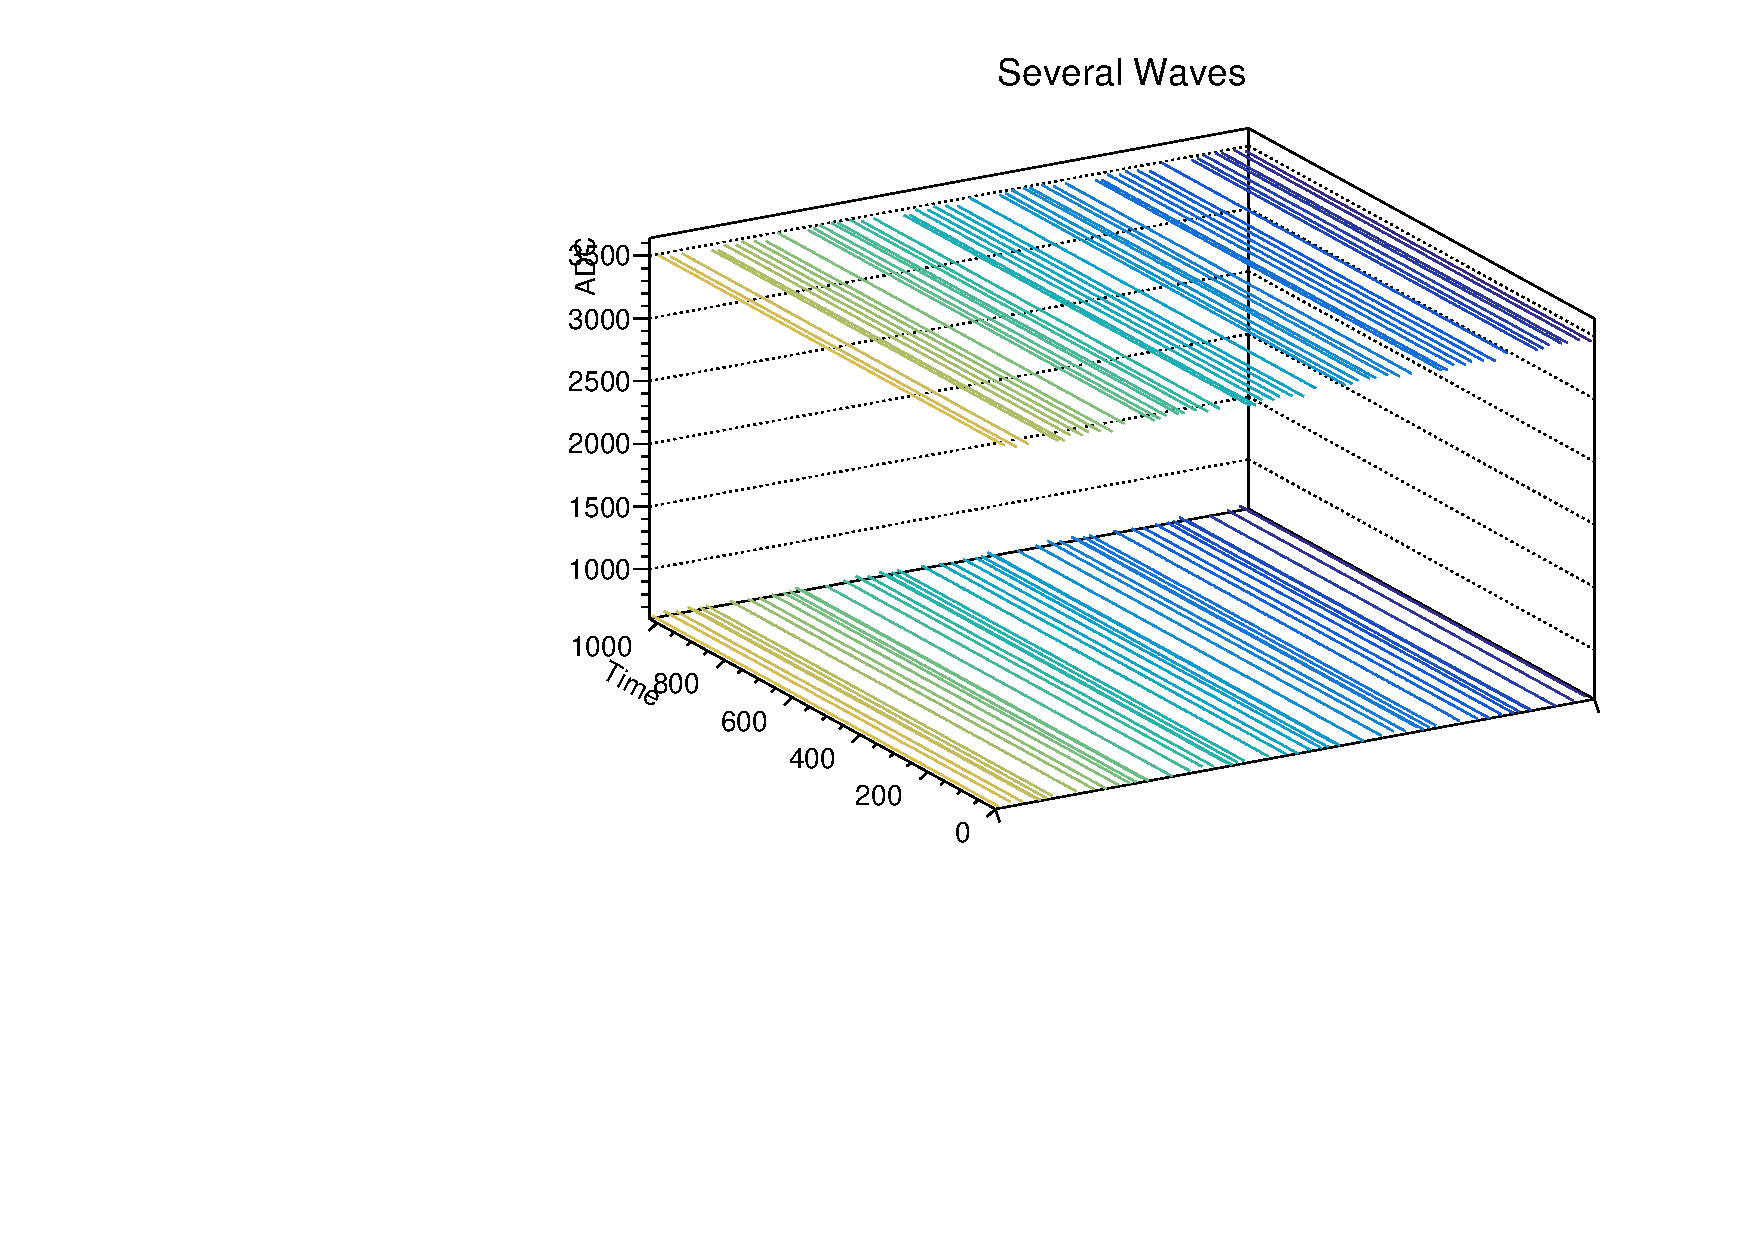
\includegraphics[width=0.85\textwidth]{240115_34_wfeb_SeveralWaves_inv.pdf}
  \caption{ADC[4:3] 连接FEB测试基线}
  \label{fig:adc34_wfeb1}
\end{figure}
FEB 中 FDA 接反的通道有:1、7、69、13、3、67、23、9、79、17、85、29、81、86、25、90、95、89、27、83、31、88、21、19、74、11、70、73、15、72、65、5、39、97、104、35、99、47、41、111、55、116、49、63、125、61、59、123、127、121、57、118、113、51、120、53、43、106、45、102、105、33、101、37。\par
ADC 各通道与 TPC 阳极条对应关系如表所示:
\begin{table}[!htbp]
  \centering
  \caption{ADC 通道与 TPC 阳极条对应关系}
  \label{tab:feb_map_tpc}
  \begin{tabular}{p{0.1\textwidth}p{0.1\textwidth}p{0.1\textwidth}p{0.1\textwidth}p{0.1\textwidth}p{0.1\textwidth}p{0.1\textwidth}p{0.1\textwidth}}
  \toprule
  ADC[0] 通道号 & TPC 阳极条 & ADC[1] 通道号 & TPC 阳极条 & ADC[2] 通道号 & TPC 阳极条 & ADC[3] 通道号 & TPC 阳极条 \\
 \midrule
  %0	  & Y55 & 32  & Y21 & 64  & Y56 & 96  & Y26 \\
  %1   & X55 & 33  & X21 & 65  & X56 & 97  & X26 \\
  %2   & Y53 & 34  & Y23 & 66  & Y52 & 98  & Y22 \\
  %3   & X53 & 35  & X23 & 67  & X58 & 99  & X28 \\
  %4   & Y57 & 36  & Y27 & 68  & Y58 & 100 & Y28 \\
  %5   & X57 & 37  & X27 & 69  & Y54 & 101 & Y24 \\
  %6   & Y59 & 38  & Y25 & 70  & A4  & 102 & X30 \\
  %7   & X59 & 39  & X25 & 71  & A6  & 103 & Y30 \\
  %8   & Y47 & 40  & Y19 & 72  & A7  & 104 & Y20 \\
  %9   & X47 & 41  & X19 & 73  & Y48 & 105 & Y16 \\
  %10  & Y45 & 42  & Y9  & 74  & X48 & 106 & X16 \\
  %11  & X45 & 43  & X9  & 75  & A5  & 107 & X20 \\
  %12  & Y49 & 44  & Y17 & 76  & X52 & 108 & X22 \\
  %13  & X49 & 45  & X17 & 77  & X50 & 109 & X18 \\
  %14  & Y51 & 46  & Y15 & 78  & Y50 & 110 & Y18 \\
  %15  & X51 & 47  & X15 & 79  & X54 & 111 & X24 \\
  %16  & Y39 & 48  & Y5  & 80  & Y38 & 112 & Y6  \\
  %17  & X39 & 49  & X5  & 81  & X38 & 113 & X6  \\
  %18  & Y37 & 50  & Y7  & 82  & Y40 & 114 & X8  \\
  %19  & X37 & 51  & X7  & 83  & X44 & 115 & Y12 \\
  %20  & Y41 & 52  & Y13 & 84  & Y44 & 116 & X12 \\
  %21  & X41 & 53  & X13 & 85  & Y42 & 117 & Y10 \\
  %22  & Y43 & 54  & Y11 & 86  & X46 & 118 & X14 \\
  %23  & X43 & 55  & X11 & 87  & Y46 & 119 & Y14 \\
  %24  & Y31 & 56  & Y1  & 88  & Y32 & 120 & Y0  \\
  %25  & X31 & 57  & X1  & 89  & Y34 & 121 & X2  \\
  %26  & Y29 & 58  & Y3  & 90  & X34 & 122 & Y2  \\
  %27  & X29 & 59  & X3  & 91  & X32 & 123 & X0  \\
  %28  & Y33 & 60  & A2  & 92  & X40 & 124 & Y8  \\
  %29  & X33 & 61  & A0  & 93  & X36 & 125 & X4  \\
  %30  & Y35 & 62  & A3  & 94  & Y36 & 126 & Y4  \\
  %31  & X35 & 63  & A1  & 95  & X42 & 127 & X10 \\
  \cellcolor[HTML]{AA0044}0	  & Y55 & \cellcolor[HTML]{AA0044}32  & Y21 & \cellcolor[HTML]{AA0044}64  & Y56 & \cellcolor[HTML]{AA0044}96  & Y26 \\
  1   & X55 & 33  & X21 & 65  & X56 & 97  & X26 \\
  \cellcolor[HTML]{AA0044}2   & Y53 & \cellcolor[HTML]{AA0044}34  & Y23 & \cellcolor[HTML]{AA0044}66  & Y52 & \cellcolor[HTML]{AA0044}98  & Y22 \\
  3   & X53 & 35  & X23 & 67  & X58 & 99  & X28 \\
  \cellcolor[HTML]{AA0044}4   & Y57 & \cellcolor[HTML]{AA0044}36  & Y27 & \cellcolor[HTML]{AA0044}68  & Y58 & \cellcolor[HTML]{AA0044}100 & Y28 \\
  5   & X57 & 37  & X27 & \cellcolor[HTML]{AA0044}69  & Y54 & \cellcolor[HTML]{AA0044}101 & Y24 \\
  \cellcolor[HTML]{AA0044}6   & Y59 & \cellcolor[HTML]{AA0044}38  & Y25 & 70  & A4  & 102 & X30 \\
  7   & X59 & 39  & X25 & \cellcolor[HTML]{AA0044}71  & A6  & \cellcolor[HTML]{AA0044}103 & Y30 \\
  \cellcolor[HTML]{AA0044}8   & Y47 & \cellcolor[HTML]{AA0044}40  & Y19 & \cellcolor[HTML]{AA0044}72  & A7  & \cellcolor[HTML]{AA0044}104 & Y20 \\
  9   & X47 & 41  & X19 & \cellcolor[HTML]{AA0044}73  & Y48 & \cellcolor[HTML]{AA0044}105 & Y16 \\
  \cellcolor[HTML]{AA0044}10  & Y45 & \cellcolor[HTML]{AA0044}42  & Y9  & 74  & X48 & 106 & X16 \\
  11  & X45 & 43  & X9  & 75  & A5  & 107 & X20 \\
  \cellcolor[HTML]{AA0044}12  & Y49 & \cellcolor[HTML]{AA0044}44  & Y17 & 76  & X52 & 108 & X22 \\
  13  & X49 & 45  & X17 & 77  & X50 & 109 & X18 \\
  \cellcolor[HTML]{AA0044}14  & Y51 & \cellcolor[HTML]{AA0044}46  & Y15 & \cellcolor[HTML]{AA0044}78  & Y50 & \cellcolor[HTML]{AA0044}110 & Y18 \\
  15  & X51 & 47  & X15 & 79  & X54 & 111 & X24 \\
  \cellcolor[HTML]{AA0044}16  & Y39 & \cellcolor[HTML]{AA0044}48  & Y5  & \cellcolor[HTML]{AA0044}80  & Y38 & \cellcolor[HTML]{AA0044}112 & Y6  \\
  17  & X39 & 49  & X5  & 81  & X38 & 113 & X6  \\
  \cellcolor[HTML]{AA0044}18  & Y37 & \cellcolor[HTML]{AA0044}50  & Y7  & \cellcolor[HTML]{AA0044}82  & Y40 & 114 & X8  \\
  19  & X37 & 51  & X7  & 83  & X44 & \cellcolor[HTML]{AA0044}115 & Y12 \\
  \cellcolor[HTML]{AA0044}20  & Y41 & \cellcolor[HTML]{AA0044}52  & Y13 & \cellcolor[HTML]{AA0044}84  & Y44 & 116 & X12 \\
  21  & X41 & 53  & X13 & \cellcolor[HTML]{AA0044}85  & Y42 & \cellcolor[HTML]{AA0044}117 & Y10 \\
  \cellcolor[HTML]{AA0044}22  & Y43 & \cellcolor[HTML]{AA0044}54  & Y11 & 86  & X46 & 118 & X14 \\
  23  & X43 & 55  & X11 & \cellcolor[HTML]{AA0044}87  & Y46 & \cellcolor[HTML]{AA0044}119 & Y14 \\
  \cellcolor[HTML]{AA0044}24  & Y31 & \cellcolor[HTML]{AA0044}56  & Y1  & \cellcolor[HTML]{AA0044}88  & Y32 & \cellcolor[HTML]{AA0044}120 & Y0  \\
  25  & X31 & 57  & X1  & \cellcolor[HTML]{AA0044}89  & Y34 & 121 & X2  \\
  \cellcolor[HTML]{AA0044}26  & Y29 & \cellcolor[HTML]{AA0044}58  & Y3  & 90  & X34 & \cellcolor[HTML]{AA0044}122 & Y2  \\
  27  & X29 & 59  & X3  & 91  & X32 & 123 & X0  \\
  \cellcolor[HTML]{AA0044}28  & Y33 & \cellcolor[HTML]{AA0044}60  & A2  & 92  & X40 & \cellcolor[HTML]{AA0044}124 & Y8  \\
  29  & X33 & 61  & A0  & 93  & X36 & 125 & X4  \\
  \cellcolor[HTML]{AA0044}30  & Y35 & \cellcolor[HTML]{AA0044}62  & A3  & \cellcolor[HTML]{AA0044}94  & Y36 & \cellcolor[HTML]{AA0044}126 & Y4  \\
  31  & X35 & 63  & A1  & 95  & X42 & 127 & X10 \\
  \bottomrule
  \end{tabular}
\end{table}
修改DataAnalysis代码发现,ADC[3] 的异常通道对应ADC[2] 的异常通道,与表中查找的不一致。经修改后得到如图\ref{fig:ADC_wfeb}所示基线。\par
\begin{figure}[htbp]
  \centering
  \begin{subfigure}[b]{0.45\textwidth}
    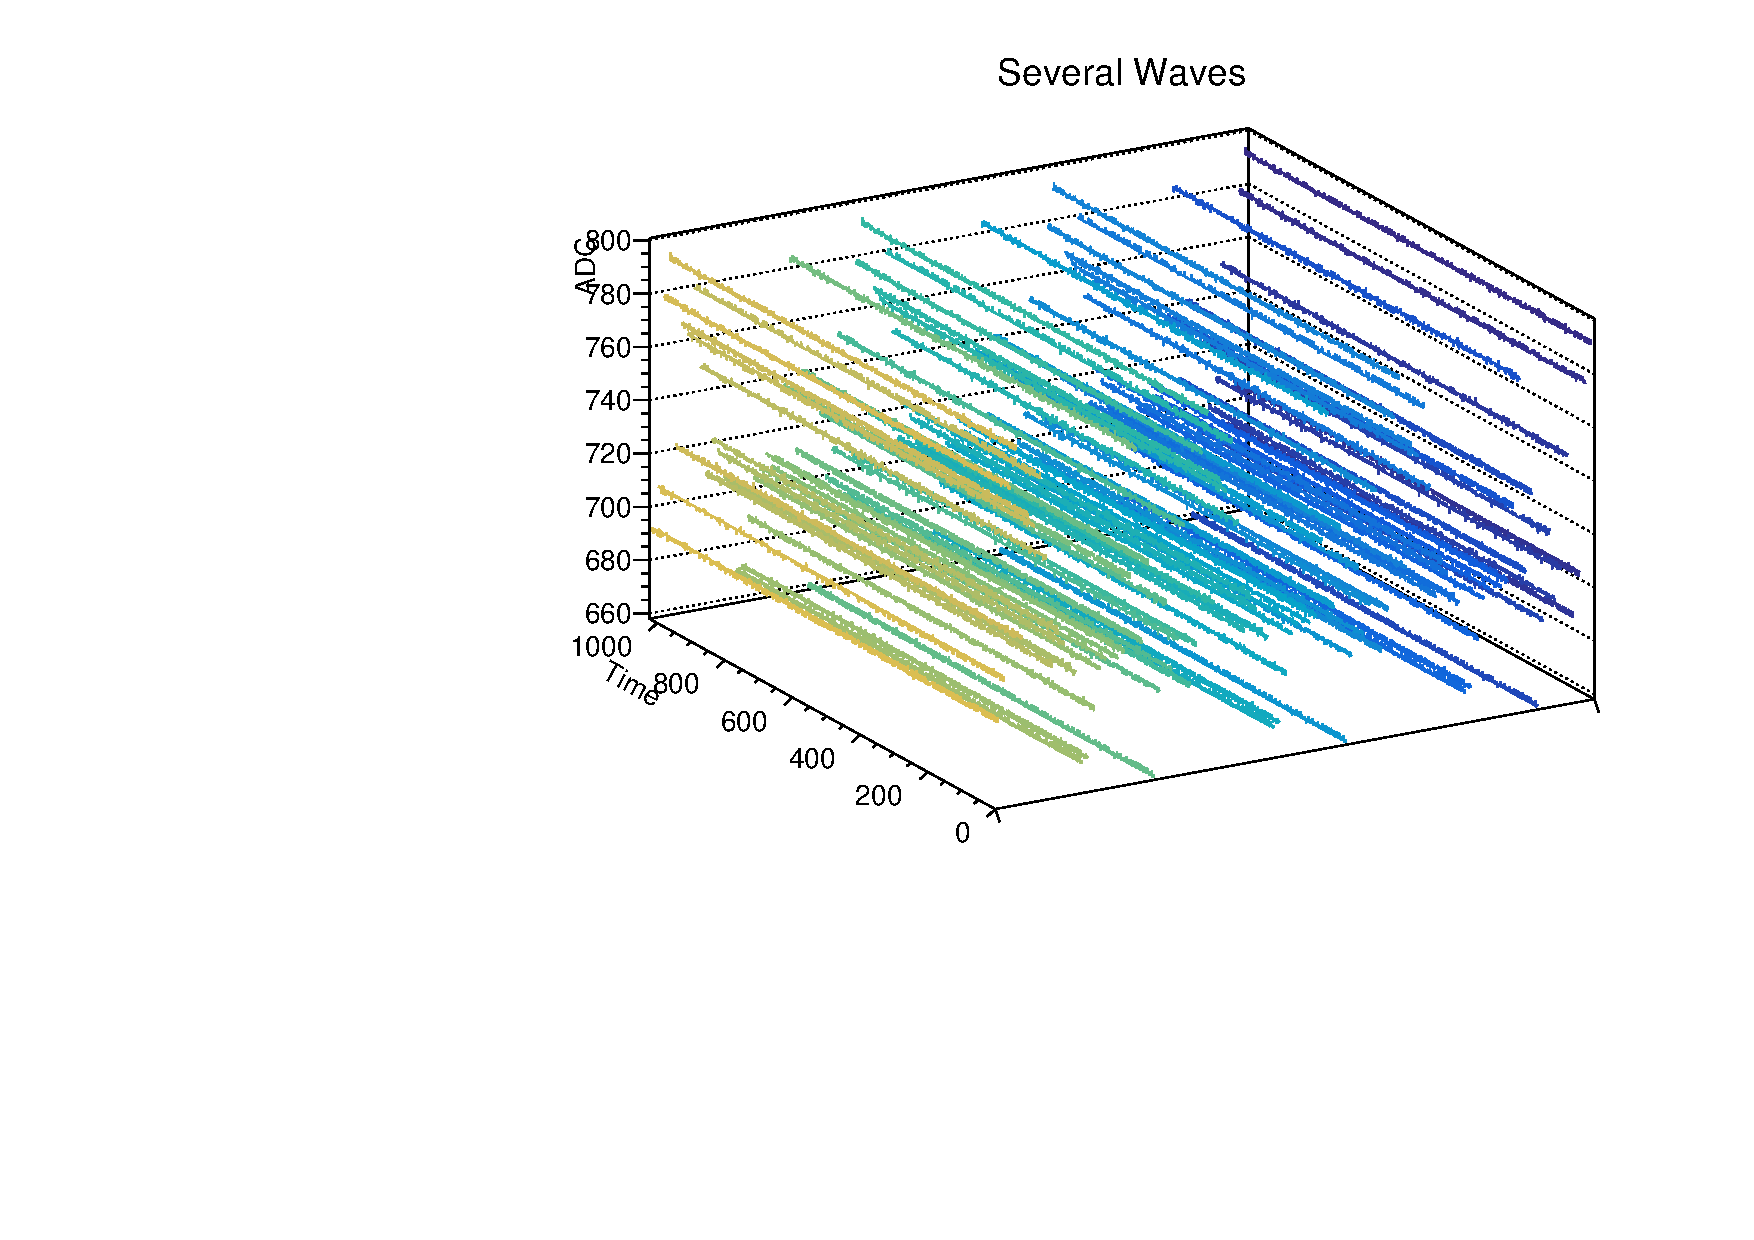
\includegraphics[width=\textwidth]{240115_12_wfeb_SeveralWaves.pdf}
    \caption{ADC[1:0] 连接FEB测试基线}
    \label{fig:adc12_wfeb}
  \end{subfigure}
  \hfill
  \begin{subfigure}[b]{0.45\textwidth}
    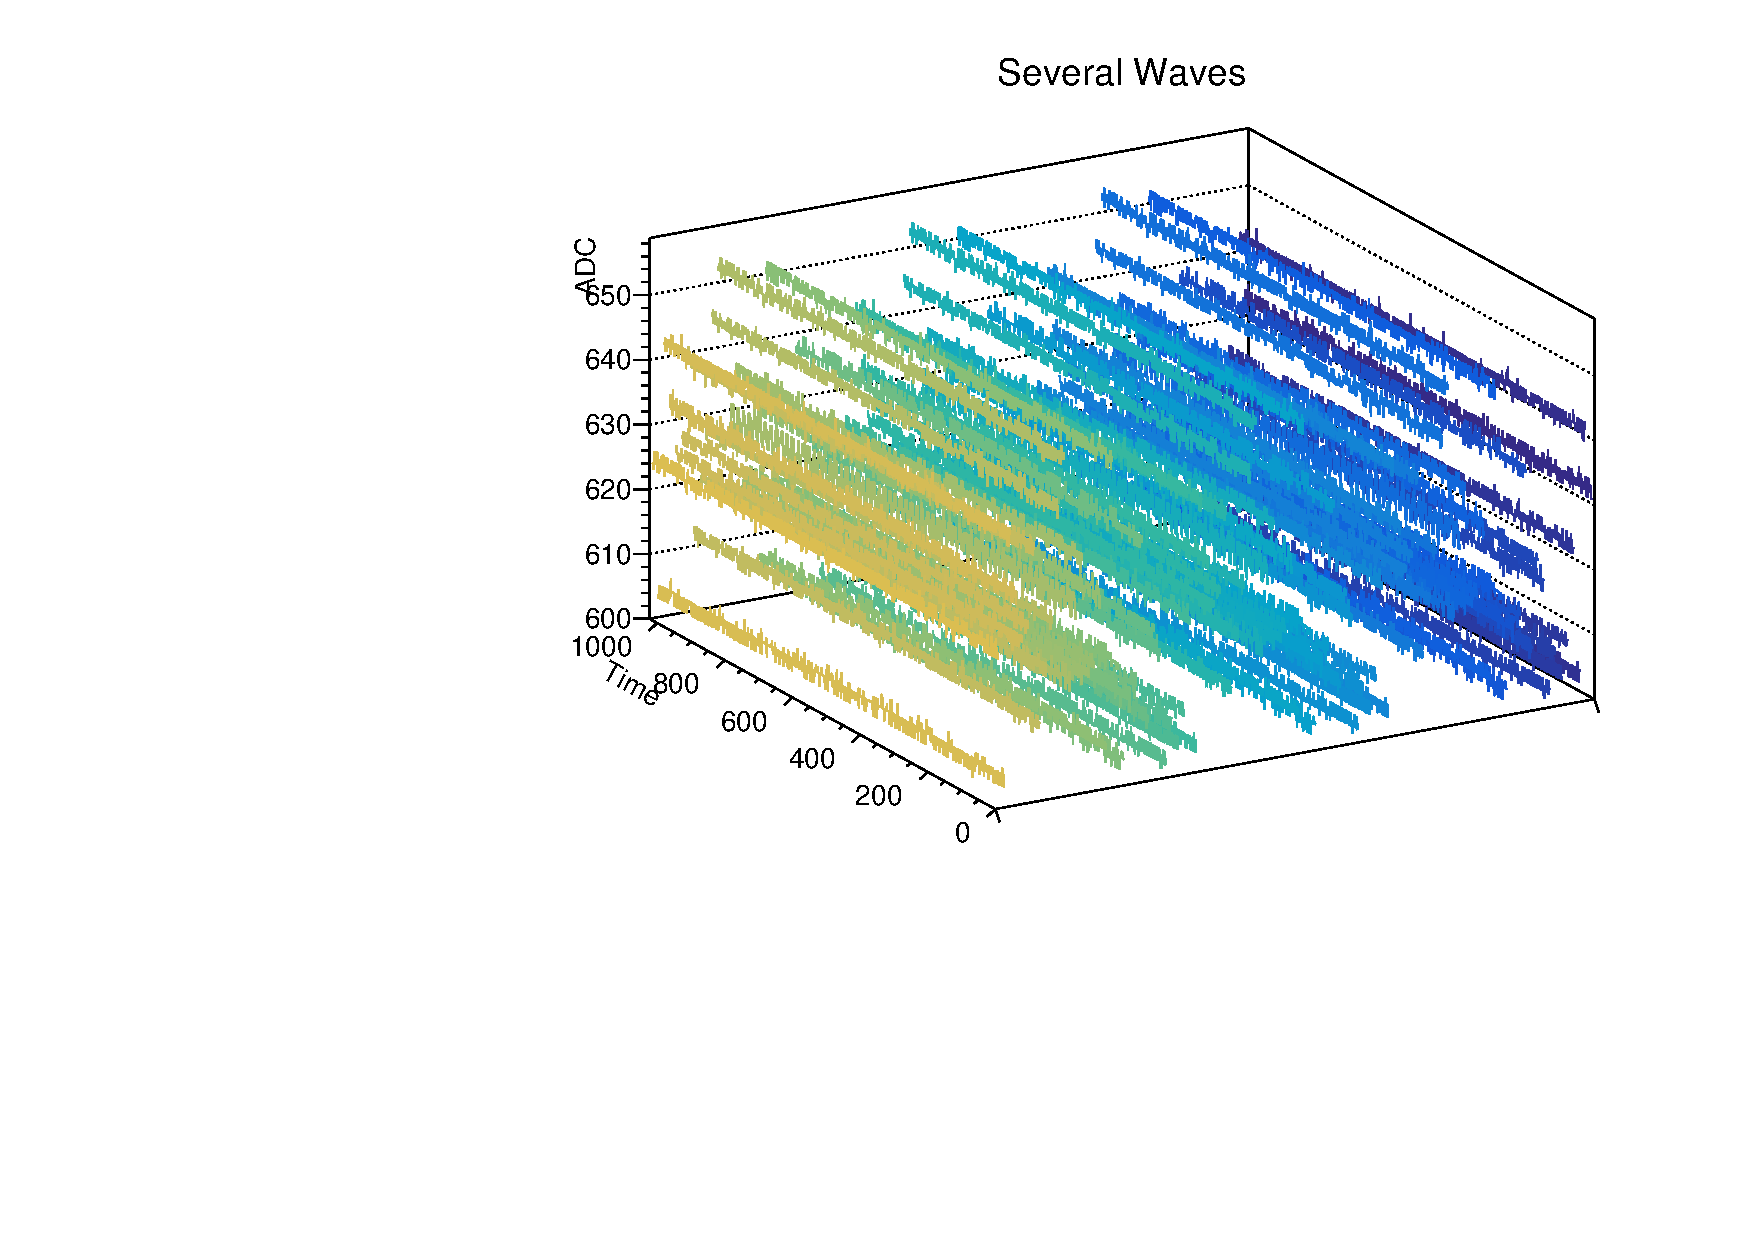
\includegraphics[width=\textwidth]{240115_34_wfeb_SeveralWaves.pdf}
    \caption{ADC[3:2] 连接FEB测试基线}
    \label{fig:adc34_wfeb}
  \end{subfigure}
  \caption{ADC 连接FEB测试基线}
  \label{fig:ADC_wfeb}
\end{figure}
